\section{METODOLOGI}

% Ubah konten-konten berikut sesuai dengan isi dari metodologi

\subsection{Data dan Peralatan/ Data dan Alat Bantu/ Material}

Penelitian ini menggunakan publik dataset yang dikumpulkan dari berbagai sumber untuk setiap kondisi otak, dengan rincian sebagai berikut:

\begin{itemize}
    \item MRI otak normal\\
          Bersumber dari \textbf{IXI Dataset} dengan jumlah citra sebanyak 578.
    \item MRI otak tumor\\
          Bersumber dari \textbf{TCIA Dataset} dengan jumlah citra sebanyak 167.
    \item MRI otak alzheimer\\
          Bersumber dari \textbf{ADNI Dataset} dengan jumlah citra sebanyak x.
    \item MRI otak stroke\\
          Bersumber dari \textbf{ATLAS Dataset} dengan jumlah citra sebanyak x.
\end{itemize}

Penelitian ini menggunakan bahasa pemrograman Python serta device yang bersumber dari cloud service google collaboratory dengan spesifikasi 2vCPU @ 2.2GHz, 13GB RAM, dan 100 GB Memory.

\subsection{Metodologi Penelitian}

    % Contoh input gambar dengan format *.jpg
    \begin{figure} [H] \centering
      % Nama dari file gambar yang diinputkan
      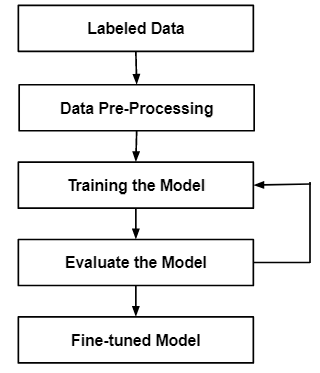
\includegraphics[scale=1]{gambar/Metodologi.png}
      % Keterangan gambar yang diinputkan
      \caption{Metodologi Penelitian}
      % Label referensi dari gambar yang diinputkan
      \label{fig:Metodologi}
    \end{figure}

Pada \emph{Metodologi} yang tertera di Gambar \ref{fig:Metodologi} terdapat 5 tahap dengan detail sebagai berikut:
\begin{outline}
    \1 Labeled Data \\
       Dataset yang digunakan dalam penelitian ini merupakan dataset citra MRI dalam bentuk 3D dengan format NifTI yang sudah memiliki label mengenai kondisi citra otak.
    \1 Data Pre-Processing \\
       Dataset yang sudah diberi label dilakukan pre-processing sebelum masuk ke dalam model agar seluruh data memiliki ukuran dan bentuk yang sama. Pre-process data ini dibagi menjadi 3 bagian yaitu:
       \2 Normalisasi nilai pixel \\
          Nilai pixel dari setiap image dilakukan proses normalisasi agar berada pada range tertentu.
       \2 Normalisasi bentuk image \\
          Bentuk 3D image dilakukan proses normalisasi agar berada pada volume dan bentuk yang sama.
       \2 Data Augmentasi
          Data dirotasi dengan sudut acak untuk menambah jumlah variasi dataset.
    \1 Training Model \\
       Pada penelitian ini model dibuat dengan menggunakan Convolution 3D layer dan Pooling 3D layer. Pada tahap ini akan melakukan percobaan terhadap jumlah layer dan tipe layer model. Selain itu pada tahap ini juga akan dicoba berbagai macam macro function yang berbeda seperti loss function, optimizer function, epoch, dan batch size pada saat training.
    \1 Evaluate Model \\
       Proses evaluasi performa model akan menggunakan confusion matrix yang dengan 4 metric perhitungan, seperti: accuracy, recall, precision, dan F1 Score.
    \1 Fine-Tuned Model \\
       Hasil akhirnya akan berupa sebuah model 3D CNN yang dapat mengklasifikasikan 4 tipe kondisi otak, yaitu: Normal, Alzheimer, Tumor, dan Stroke.
\end{outline}